\chapter{Latex}

15/12/2017:

Hôm nay tự nhiên nổi hứng vẽ hình trên latex. Thấy blog này là một guide line khá tốt về viết blog phần mềm. Quyết định cài latex

Theo [hướng dẫn này](http://milq.github.io/install-latex-ubuntu-debian/)

```
sudo apt-get install texlive-full
sudo apt-get install texmaker
```

Tìm được ngay bên này https://www.overleaf.com/ có vẻ rất hay luôn

Hướng dẫn cực kì cơ bản http://www.math.uni-leipzig.de/~hellmund/LaTeX/pgf-tut.pdf

Chương trình đầu tiên, vẽ diagram cho LanguageFlow

\begin{lstlisting}[language=text]
\documentclass[border=10pt]{standalone}
\usepackage{verbatim}
\begin{comment}
\end{comment}
\usepackage{tikz}
\begin{document}
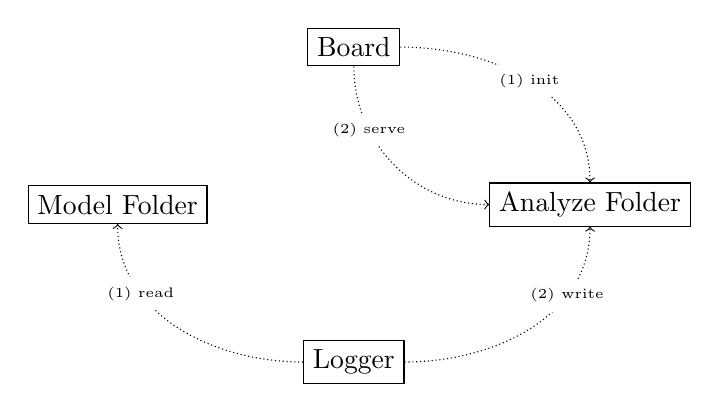
\begin{tikzpicture}
    \node[draw] (model) at (0, 0) {Model Folder};
    \node[draw] (analyze) at (6, 0) {Analyze Folder};
    \node[draw] (board) at (3,2) {Board};
    \node[draw] (logger) at (3, -2) {Logger};

    \path[->, densely dotted] (board.east)
    	edge [out=0, in=90]
    	node[fill=white, pos=.5] {\tiny (1) init}
        (analyze.north) ;
    \path[->, densely dotted] (board.south)
    	edge [out=-90, in=180]
    	node[fill=white, pos=.3] {\tiny (2) serve}
        (analyze.west) ;
	\path[->, densely dotted] (logger.west)
    	edge [out=180, in=-90]
    	node[fill=white, pos=.7] {\tiny (1) read}
        (model.south) ;
	\path[->, densely dotted] (logger.east)
    	edge [out=0, in=-90]
    	node[fill=white, pos=.7] {\tiny (2) write}
        (analyze.south) ;
\end{tikzpicture}
\end{document}
\end{lstlisting}

Doc! Doc! Doc! https://en.wikibooks.org/wiki/LaTeX/PGF/TikZ